\chapter{Carbon Dioxide Splitting}

\section{Traditional Process}

Before understanding the process of plasma-assisted CO$_2$ splitting, it would be useful to briefly explain the traditional thermally driven process. An ideal form of the decomposition would simply be the reverse of the coal burning process, shown in equation \ref{ce:ideal_co2_splitting}. This is similar to the process of methane (CH$_4$) pyrolysis, a method of generating hydrogen gas that has been successfully done in industry. The reaction for CH$_4$ pyrolysis is shown in equation \ref{ce:ch4_pyrolysis}.

\begin{equation}
    \ce{CO_2 (g) -> C (s) + O_2 (g)}
    \label{ce:ideal_co2_splitting}
\end{equation}

\begin{equation}
    \ce{CH_4 (g) -> C (s) + 2H_2 (g)}
    \label{ce:ch4_pyrolysis}
\end{equation}

However, such ideals are not currently feasible due to the incredible stability of the CO$_2$ molecule, with a Gibbs free energy of formation ($\Delta G^\circ$) of -394 kJ mol$^{-1}$. This is significantly higher than most other common gases as illustrated in figure \ref{fig:co2_stability}. As such, there is limited successful research on a viable process.

\begin{figure}[h!]
	\centering
	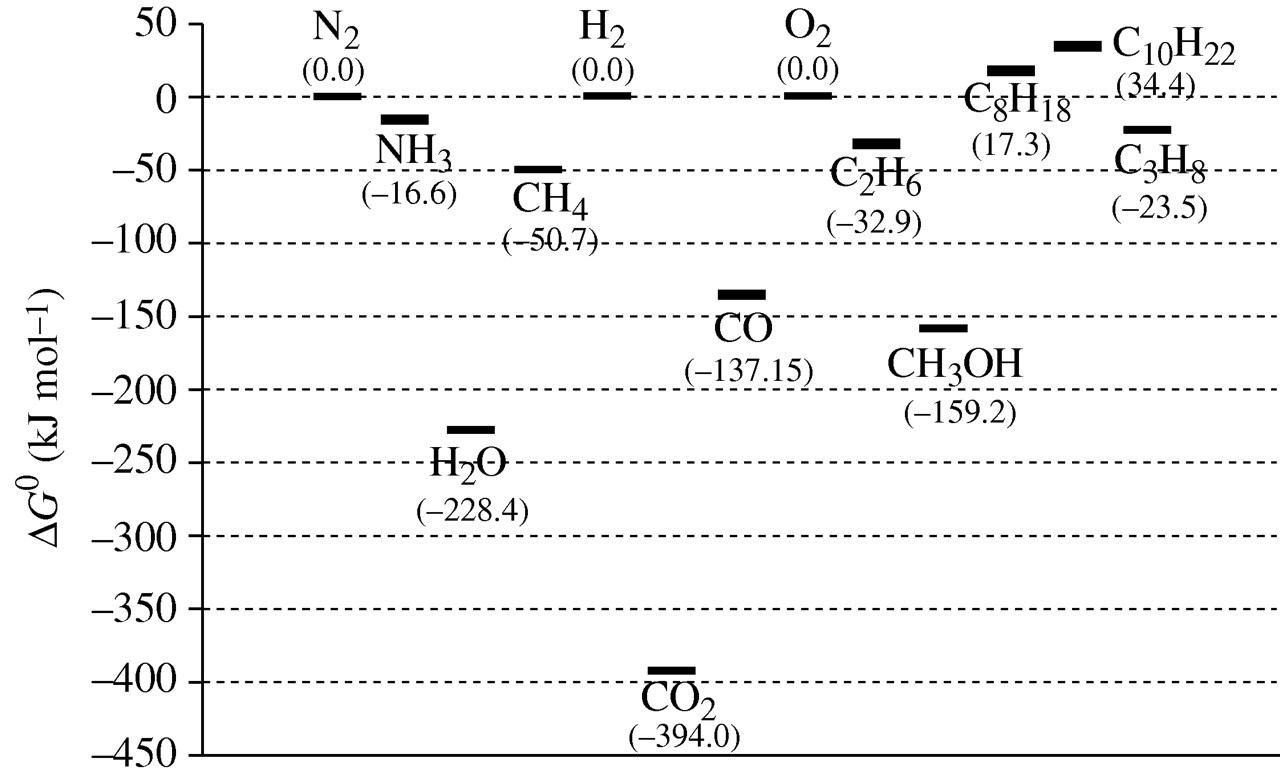
\includegraphics[width=0.8\linewidth]{chapter_3/figures/co2_stability.jpg}
	\caption{Gibbs free energy of formation for different chemicals based on data from the NIST database. \cite{jiang_xiao_kuznetsov_edwards_2010}}
	\label{fig:co2_stability}
\end{figure} 

\newpage

Instead, current CO$_2$ splitting processes in the literature typically involves splitting the molecule into carbon monoxide (CO) and atomic oxygen (O). This reaction is slightly more viable than the ideal decomposition process, with an enthalpy change of $\Delta H = 283 $ kJ mol $^{-1}$. This reaction is shown in equation \ref{eq:co2_splitting}.

\begin{equation}
    \ce{CO_2 (g) -> CO (g) + \frac{1}{2}O_2 (g)}
    \label{eq:co2_splitting}
\end{equation}

In the thermally driven process, CO$_2$ dissociated into CO begins at around 2000, forming primarily oxygen gas; but can also from atomic O at around 2300K \cite{Snoeckx2017, Centi2021}. Figure \ref{fig:thermal_co2_conversion} highlights this conversion based on temperature, along with its corresponding energy efficiency. For reference, converting the remaining CO to pure carbon via the Boudouard catalytic disproportionation reaction requires around 6300K \cite{Centi2021}. 

\begin{figure}[h!]
	\centering
	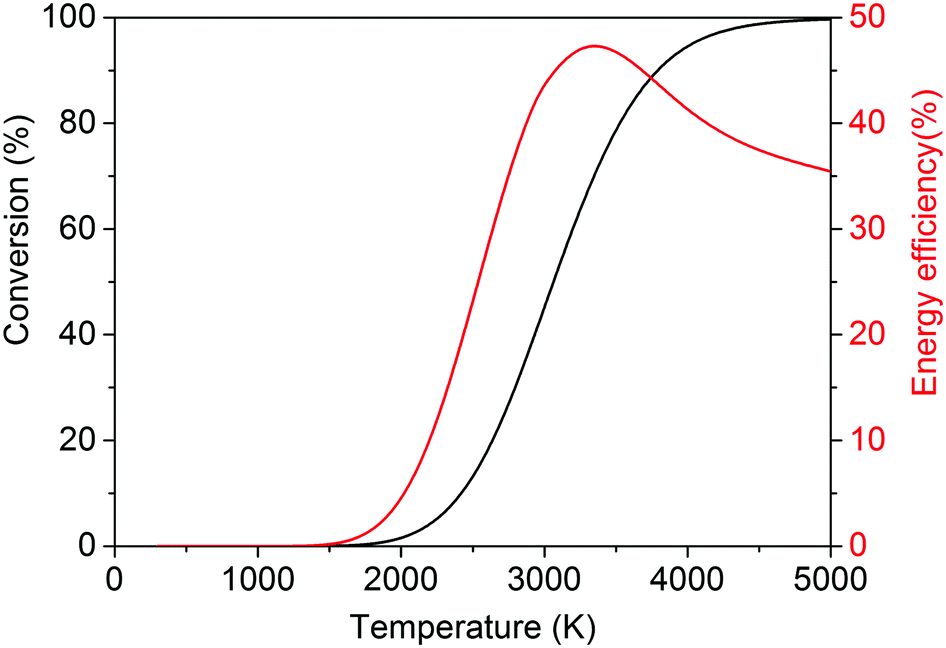
\includegraphics[width=0.7\linewidth]{chapter_3/figures/thermal_co2_conversion.png}
	\caption{Thermal conversion and energy efficiency of CO$_2$ splitting as a function of temperature. \cite{Snoeckx2017}}
	\label{fig:thermal_co2_conversion}
\end{figure}

It is no surprise why CO$_2$ splitting is greatly benefited with the use of catalysts, though this also increase the costs and complexity. The former is self explanatory, but the reason for increased complexity is that oxygen tends to remain on the catalyst surface, thus reducing its activity over time \cite{Shin2017}. 

As a result, it is oftentimes more practical to include the use of a co-reactant to undergo the decomposition process. Ideally, this is done using a co-reactant with a higher Gibbs free energy (i.e. a less negative value) \cite{jiang_xiao_kuznetsov_edwards_2010}. In the literature, the most common co-reactants for CO$_2$ splitting are CH$_4$ ($\Delta G^\circ$ = -50.7 kJ mol$^{-1}$) and hydrogen gas (H$_2$, $\Delta G^\circ$ = 0.0 kJ mol$^{-1}$). A brief overview of both these co-reactant proesses are detailed below.

CH$_4$ is fairly abundant, and one common use of it is for the process of steam methane reforming (involving CH$_4$ + H$_2$O) to produce syngas (CO + H$_2$). Syngas is typically in intermediary for the production of ammonia, however is also used to produce liquid hydrocarbons via the Fischer–Tropsch process. Hence, it is no surprise why there has been research into investigating CO$_2$ reformation of CH$_4$. This process is known as the dry reforming of methane, which is an endothermic reaction requiring $\Delta H  = 247.3$ kJ mol$^{-1}$. 

\begin{equation}
    \ce{CH_4 + CO_2 -> 2CO + 2H_2}
    \label{eq:drm}
\end{equation}

To push the equation to the right, high temperatures (between 1000-1300 K) are required and typically done in the presence of a catalysts \cite{pakhare_spivey_2014}. Many different catalyst have been looked at, including the use of noble metals such as Rhodium (Rh) and Ruthenium (Ru), which have shown high activity and stability \cite{Rezaei2006, Rostrup-Nielsen1993}. However due to costs, most research has been into nickel (Ni) based catalysts which has been shown to have a similar activity to the noble metals \cite{Ma2009}. Regardless of catalyst used, the big limitation with this process is the formation of soot on the catalyst, reducing the yields.

Besides the production of syngas, there are other uses for CH$_4$. The most common use of CH$_4$ by far is as a fuel source as it is the major constituent of natural gas. While not being particularly green in the long term, one viable use in the intermediary is to take excess electricity generated from renewable sources and convert them into synthetic CH$_4$. This is an example of the Sabatier reaction, and has been in operation at a power-to-gas plant in Germany for nearly a decade \cite{etogas}.

\begin{equation}
    \ce{CO_2 + 4H_2 -> CH_4 + 2H_2O}
    \label{eq:sabatier_reaction}
\end{equation}

The benefit of this reaction is that is exothermic, with a $\Delta H = -165.3$ kJ mol$^{-1}$, but it does require a catalyst in order to achieve high conversion yields. Nonetheless, there are two issues with this process. The first has to do with the fact that most of the world's supply of H$_2$ comes from the process of steam methane reforming, which uses CH$_4$ in the first place. The other issues is that unless water is the desired end product, a third of the H$_2$ used goes towards the creation of a waste product; not ideal when using this process at scale. 

One case where water is the desired end product is on board the International Space Station, where NASA uses the Sabatier reaction to produce water for consumption by the astronauts \cite{the_sabatier_system}. The excess CH$_4$  is simply released into space. The reaction for this is expressed as:

\begin{equation}
    \ce{2H_2O ->[ electrolysis ] O_2 + 2H_2 ->[ respiration ] CO_2 + 2H_2 + 2H_2 (added) -> 2H_2O + CH_4 }
\end{equation}

Though even for this, half the hydrogen in the Sabatier reaction comes from resupply missions from Earth.


\newpage



%This though is a simplification of the process, as it is most likely a two part mechanism \cite{rayne_2008}. The first half of the process would involve splitting the CO$_2$ into carbon monoxide (CO) and atomic oxygen (O) as seen in \ref{eq:co2_splitting}. The second step could take one of two possible pathways, however the most likely of the two would be the Boudouard reaction, seen in \ref{eq:boudouard_reaction}; however, this specific reaction is beyond the scope of this report.
%
%\begin{equation}
%    \ce{2CO_2 -> 2CO + O_2}
%    \label{eq:co2_splitting}
%\end{equation}
%\begin{equation}
%    \ce{2CO -> C + CO_2}
%    \label{eq:boudouard_reaction}
%\end{equation}
%
%Traditional thermal CO$_2$ splitting has not had much success to date, primarily due to the fact that CO$_2$ is an incredibly stable molecule with a Gibbs free energy of formation ($\Delta G^\circ$) of -394 kJ mol$^{-1}$. 
%
%The enthalpy of formation ($\Delta H^\circ_f$) of the reaction in \ref{eq:co2_splitting} is +283 kJ mol$^{-1}$, meaning that it is endothermic. Thus in order to make this reaction favourable, high temperatures are required. Figure \ref{fig:thermal_co2_conversion} highlights the conversion of such a reaction based on temperature, along with its corresponding energy efficiency \cite{Snoeckx2017}. This process could be improved by the presence of an active catalysts but this also increase the complexity and costs. 
%%Alternatively, one could remove the reactants
%
%\begin{figure}[h!]
%	\centering
%	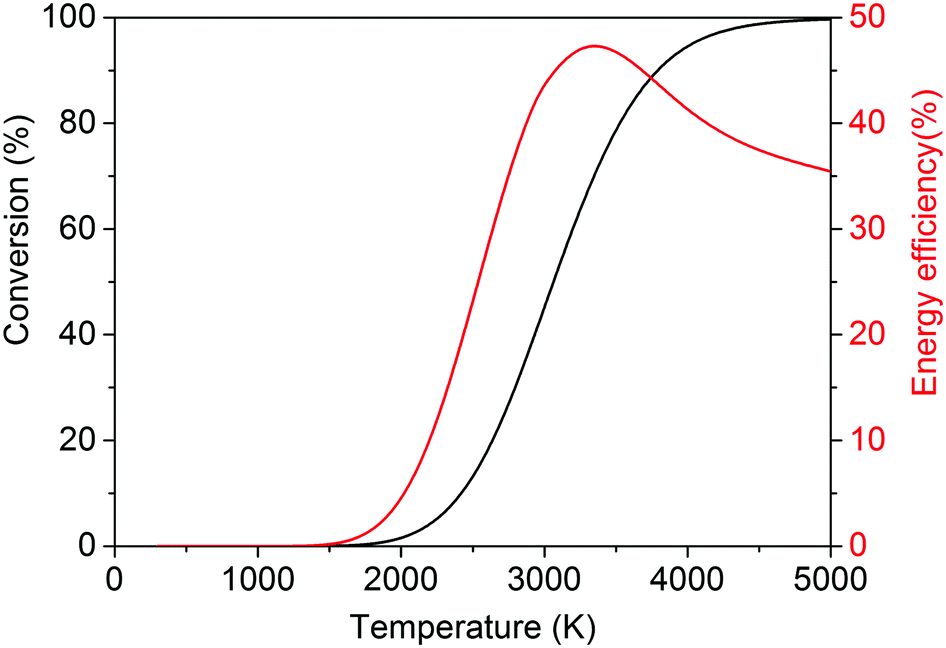
\includegraphics[width=0.6\linewidth]{chapter_3/figures/thermal_co2_conversion.png}
%	\caption{Thermal conversion and energy efficiency of CO$_2$ splitting as a function of temperature. \cite{Snoeckx2017}}
%	\label{fig:thermal_co2_conversion}
%\end{figure}
%
%Because of the low energy efficiency of pure CO$_2$ splitting, it is oftentimes more practical to include the use of a co-reactant. Ideally, this is done using a co-reactant with a higher Gibbs free energy (i.e. a less negative value) \cite{jiang_xiao_kuznetsov_edwards_2010}. In the literature, the most common co-reactants for CO$_2$ splitting are methane (CH$_4$, $\Delta G^\circ$ = -50.7 kJ mol$^{-1}$) and hydrogen (H$_2$, $\Delta G^\circ$ = 0.0 kJ mol$^{-1}$).




%
%
%As for using H$_2$ as a co-reactant to CO$_2$ splitting, this process is known as the Sabatier reaction. The reaction, seen in \ref{eq:sabatier_reaction}, is typically to generate synthetic natural gas but has other uses such as the production of water on the international space station \cite{the_sabatier_system}.
%
%\begin{equation}
%    \ce{CO_2 + 4H_2 -> CH_4 + 2H_2O}
%    \label{eq:sabatier_reaction}
%\end{equation}
%
%The reaction is exothermic, with a $\Delta H^\circ_f$ = -165.3 kJ mol$^{-1}$, but does require a catalyst in order to achieve high conversion yields. Nonetheless, there are two issues with this process. The first being, unless water is the desired end product, a third of the H$_2$ used goes towards the creation of a waste product; not ideal when using this process at scale. The other issues has to do with the fact that most of the world's supply of H$_2$ comes from the process of steam reforming, which produces CO$_2$ as a by-product. 

\newpage
\section{Plasma-assisted CO$_2$ Splitting}

As highlighted above, there are several shortfalls with the traditional process of CO$_2$ splitting. This is where the use of plasma, specifically non-thermal plasmas (i.e. generated by electric means), can be beneficial. In these plasmas,  electrons have a higher temperature than the ions or the background gas. Energetic electrons in the plasma can dissociate molecules, even highly stable ones such as CO$_2$ at standard temperatures and pressures \cite{Snoeckx2017}. 

Because of this behaviour, there is no need for heat and pressurised reactors, reducing the complexity (and thereby costs). This leads on to the second benefit, where the entire operation of such a reaction is described as a 'turn-key' process due to the ability to instantly turn the plasma on and off, with minimal stabilisation times. There is also no need for rare earth metals to be used as catalysts, and it has been shown that plasma reactors can have good scalability as shown by Kogelschatz in \cite{kogelschatz_2003}. 

For the plasma assisted decomposition process, there are several pathways available for the reaction to take place. Just to note, all reactions will have the units eV, rather than kJ mol$^{-1}$, henceforth as it is the commonly used nomenclature in the literature. For reference, the CO$_2$ splitting reaction shown in equation \ref{eq:co2_splitting} requires about 2.93 eV.

The dominant pathway is via electron-impact dissociation, with an energy threshold around 5.5 eV per molecule; which corresponds to the energy required to break the \ce{C=O} bond \cite{Bogaerts2020};. This is often accompanied by the recombination of the oxygen atoms \cite{Chen18}. This is shown in equations \ref{ce:electron_dissociation} and \ref{ce:oxygen_recombination} respectively.

\begin{equation}
    \ce{CO_2 + e^{-} -> CO + O + e^{-}}
    \label{ce:electron_dissociation}
\end{equation}

\begin{equation}
    \ce{M + O + O -> O_2 + M}
    \label{ce:oxygen_recombination}
\end{equation}

Note that M is a particle from the background gas.

\newpage

Though, it is also possible splitting to occur when vibrationally excited CO$_2$ molecules collide with the atomic oxygen or electrons, requiring around 0.3 eV and less than 1 eV per molecule respectively \cite{Chen18}. These are also shown in equations \ref{ce:vibrational_exitation_oxygen} and \ref{ce:vibrational_exitation_electron} respectively.

\begin{equation}
    \ce{CO^*_2 + O -> CO + O_2}
    \label{ce:vibrational_exitation_oxygen}
\end{equation}

\begin{equation}
    \ce{CO^*_2 + e^{-} -> CO + O + e^{-}}
    \label{ce:vibrational_exitation_electron}
\end{equation}

There are several different methods to generate plasma for CO$_2$ splitting in the literature, however the most common are: dielectric barrier discharges (DBD), gilding arc discharges (GA), and radio frequency (RF)/microwave (MW) discharges. These different processes used are typically characterised and evaluated by two main parameters: the \textit{conversion efficiency} and the \textit{energy efficiency}. The conversion efficiency ($\rchi_{CO_2}$) simply denotes the fraction of CO$_2$ used by the splitting process, and can be defined as:

\begin{equation}
    \rchi_{CO_2} = \frac{n_{start} - n_{end}}{n_{start}}
\end{equation}

where $n$ is the number of moles of CO$_2$. Though oftentimes, it is easier to determine the conversion efficiency based on the yields of the product.

On the other hand, energy efficiency ($\eta_{CO_2}$) corresponds to the fraction of input energy that went into splitting the CO$_2$ molecules. This can be expressed as:

\begin{equation}
    \eta_{CO_2} = \frac{\rchi_{CO_2} \Delta H^{\circ}_{CO_2, 298K}}{SEI}
\end{equation}

where $SEI$ is the specific energy input, which describes the average energy available per molecule in the plasma that contribute to plasma chemical reactions \cite{Hegemann2023}. The SEI can be calculated as the ratio between the discharge power and the gas flow rate. The discharge power is almost always measured in watts (W), however there are many different standard units for measuring flow rates of gases. 

In this report, all flow rates are measured in standard cubic centimetres per minute (sccm). With discharge power (P) and flow rate (Q), the SEI (in eV molecule$^{-1}$) can be calculated as follows \cite{Ozkan2015}:

\begin{equation}
    SEI = \frac{P \text{ (Js$^{-1}$)}}{Q \text{ (cm$^{3}$ min$^{-1}$)}} \times \frac{60 \text{ (s min$^{-1}$)} \times 6.24 \times 10^{18} \text{(eV J$^{-1}$)} \times 24000 \text{ (cm$^{3}$ mol$^{-1}$)}}{6.022 \times 10^{23} \text{ (molecules mol$^{-1}$)}}
\end{equation}

Note that the value 24000 cm$^{3}$mol$^{-1}$ is derived from the ideal gas law at atmospheric pressure and at 293K. 

Snoeckx and Bogaerts compiled a list of various plasma reactors for CO$_2$ conversion, and evaluated their conversion and energy efficiencies \cite{Snoeckx2017}. An illustration of the result can be seen in figure \ref{fig:conversion_and_energy_efficiencies}. 

\begin{figure}[h!]
	\centering
	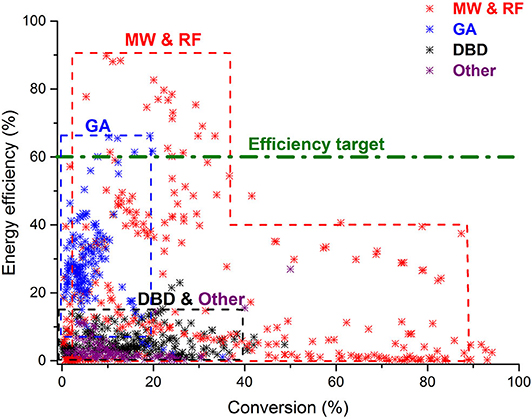
\includegraphics[width=0.6\linewidth]{chapter_3/figures/conversion_and_energy_efficiencies.jpg}
	\caption{Comparison of conversion and energy efficiencies for various CO$_2$ splitting plasma reactors \cite{Snoeckx2017}.}
	\label{fig:conversion_and_energy_efficiencies}
\end{figure}

From the figure \ref{fig:conversion_and_energy_efficiencies}, it is evident that one of the most extensively studied processes for CO$_2$ splitting involved DBD reactors. This is not surprising given that DBD reactors have already had industrial success in areas related to ozone production and VOC removal \cite{Kogelschatz2003}. Nonetheless, they seem to have relatively poor performance, which makes it hard to justify them for industrial applications. GA plasma perform better than DBD reactors when it comes to energy efficiency. However, they struggle to get a conversion efficiency greater 20\%, most likely due to the fact that the amount of gas passing through the the arc of plasma is minimal.

RF and MW plasmas by contrast appear to have a wide spectrum of results. From reactors that trade off low conversion for high energy efficiencies and vice versa, to designs that are located in the middle of both parameters. Though, a lot of these RF and MW plasma reviewed operated at sub-atmospheric pressure. Nevertheless, because of the promise shown by MW reactors, the rest of this chapter will highlight examples from the literature.

One final thing to note from figure \ref{fig:conversion_and_energy_efficiencies} is the inclusion of an energy efficiency target of 60\%. Snoeckx and Bogaerts believe that this values should be the target for plasma assisted splitting to be competitive and worthy alternative to traditional methods. The rational behind this number was two fold. First was a comparison to electrochemical water splitting, which have energy efficiencies of approximately 65-75\%. The next was to couple CO$_2$ splitting with solar energy, to give a solar-to-fuel conversion efficiency around 20\%, which was said to be competitive in industry. 

Many experiments utilise a structure as seen in figure \ref{fig:mw_reactor}, called surface-wave discharges. Gas is typically fed through a tube (typically quartz), coupled with an external wave guide where the microwave discharge is generated. The typical frequencies in such experiments are 915 MHz or 2.45 GHz, which are comparable by the dimensions of the setup. 

\begin{figure}[h!]
	\centering
	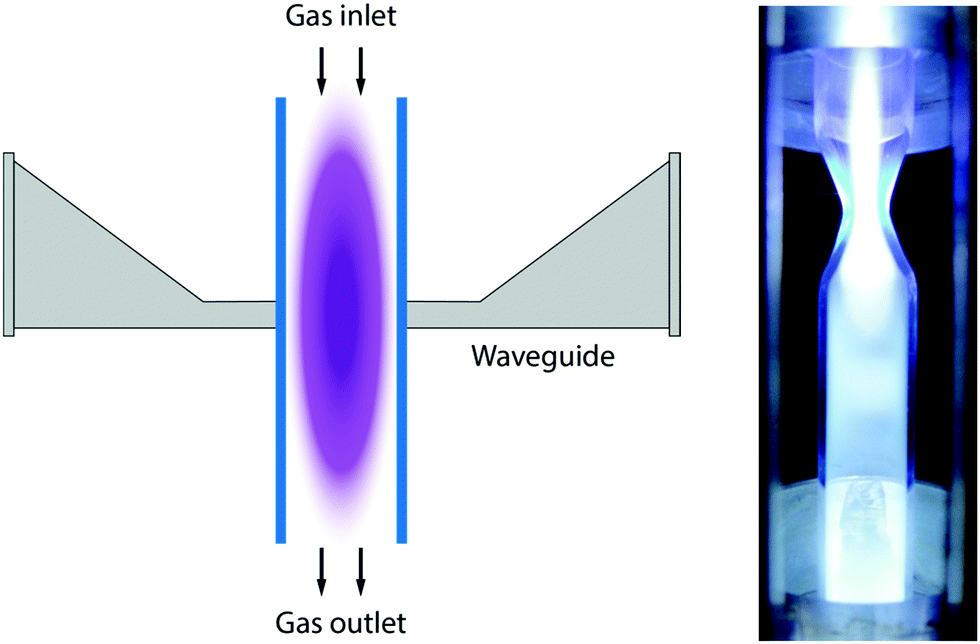
\includegraphics[width=0.75\linewidth]{chapter_3/figures/mw_reactor.png}
	\caption{Schematic of microwave reactors for CO$_2$ splitting \cite{Snoeckx2017}.}
	\label{fig:mw_reactor}
\end{figure}

Bongers et al used such a reactor \cite{Bongers2015DevelopmentsIC} at a frequency of 915 MHz at approximately 150 Torr. They were able to obtain an conversion efficiency of up to 23\% at an energy efficiency of 36\%, through were able to achieve an energy efficiency of 50\% at lower powers which reduced the conversion. The downside of their setup was that it required a specialised configuration where the gas was supersonically expanded in the plasma.

\newpage

A more typical configuration was done by Silva et al \cite{Silva2014}, the experiment was operated at 2.45 GHz with a pulsed microwave generator, but it was operating at a very low pressure (between 1-10 Torr). They used a gas mixture of CO$_2$ with 5\% nitrogen (N$_2$), and were able to get conversion efficiency of 80\% with a steady energy efficiency of around 12\%. 

It is common to see co-reactants with plasma-assisted CO$_2$ splitting for the same reason as the thermally driven process, it becomes much easier for the reaction to take place because of thermodynamics. Generally, inert gases such as Argon (Ar) or Helium (He) are used. However, it is also common to see N$_2$ due to its abundance and cost effectiveness. The flaw with using N$_2$ is that the conversion of N$_2$ is more abundant than CO$_2$, resulting in the formation of undesirable gases such as NO$_2$, NO, and N$_2$O \cite{Qin2018}.  

The rational for using inert gases is to function as an electron source, allowing for the plasma to be sustained more easily. It has also been shown that the breakdown voltage decreases when CO$_2$-Ar or CO$_2$-He mixtures are used \cite{Ramakers2015}, and that the electron density increases promoting more frequent collisions \cite{Qin2018, Ramakers2015}. When choosing between the two gas inert gases, Ar is cheaper than He. However, He has a higher ionising potential (of 24.6 eV) compared to that of Ar (of 15.8 eV), which explains why He plasmas have a higher electron temperature \cite{Qin2018, Jeroen_Jonkers_2003}.

Other gases have been used as co-reactants, such as H$_2$ by Chen et al \cite{chen2017role}. They used a surface waveguide with a frequency of 915 MHz, at a pressure of around 30 Torr. The H$_2$ is actually first produced from the decomposition of water (H$_2$), then the following reaction takes place:

\begin{equation}
    \ce{CO$_2$ (g) + H$_2$ (g) -> CO (g) + H$_2$O (g)}
\end{equation} 

They were able to obtain a 22\% conversion efficiency and a 52\% energy efficiency. These efficiencies were obtained with the use of a (NiO/TiO) catalyst.

Additionally, CH$_4$ has been used co-reactants by Chun et al \cite{Chun2017}. They used a plasma torch operating at 2.45 GHz, which has a similar structure to the surface waveguides shown in figure \ref{fig:mw_reactor} but channels have been made within the quartz tube to allow the gas to swirl. With this, they were able to get conversion efficiencies of 68.4\% for CO$_2$ and 96.8\% for CH$_4$. No energy efficiency was given, but some rough calculations based on parameters used gives an efficiency of around 33\%. The big advantage of this process had to do with the fact that it is one of the few processes that operates at atmospheric pressure (760 Torr).


%Such a design was used by Spencer and Gallimore \cite{spencer_gallimore_2010} to achieve a conversion efficiency of approximately 90\%; although this came at the cost of energy efficiency which reached a maximum of 3\%. The authors went on to state that such a system would not be suitable for  CO$_2$ emission reductions.

So far all the previous examples include the use of gaseous reactants. It is also possible to for the co-reactants for the CO$_2$ decomposition process to be liquids. Research into this was limited due to the fact that these liquids are typically organic liquids which made them unsuitable at low pressure operations (as seen with many of the previous examples) due to vapor pressure limitations \cite{Bruggeman2016}. However, with the advances in microwave reactors operating at atmospheric pressure, these plasma–liquid systems have become a viable area of research. The obvious advantage is that this leads to even more possible reactions with CO$_2$ to produce desired end products. Additionally, if the end product is also a liquid, it allows for easier separation of the product from the waste reactants. 

One example of research into plasma–liquid systems was done by Gorbanev et al \cite{Gorbanev2017}. They tested three different organic solutions (dehalogenation of iodoarenes, 5-exo-trig cyclisation, and trifluoromethylation with the Togni-II reagent) using a frequency of 24.9 kHz. The apparatus used was similar to that in figure \ref{fig:mw_reactor}, but because the frequency used was RF, the tube was modified to include embedded electrodes. The feed gas included a CO$_2$-He mixture, with yields of up to 95\% after 30 mins for the last test case. Though, there were a lot of variations in the results, and even the authors note that the results are only preliminary with more work required to optimise reaction efficiency.

\begin{figure}[h!]
	\centering
	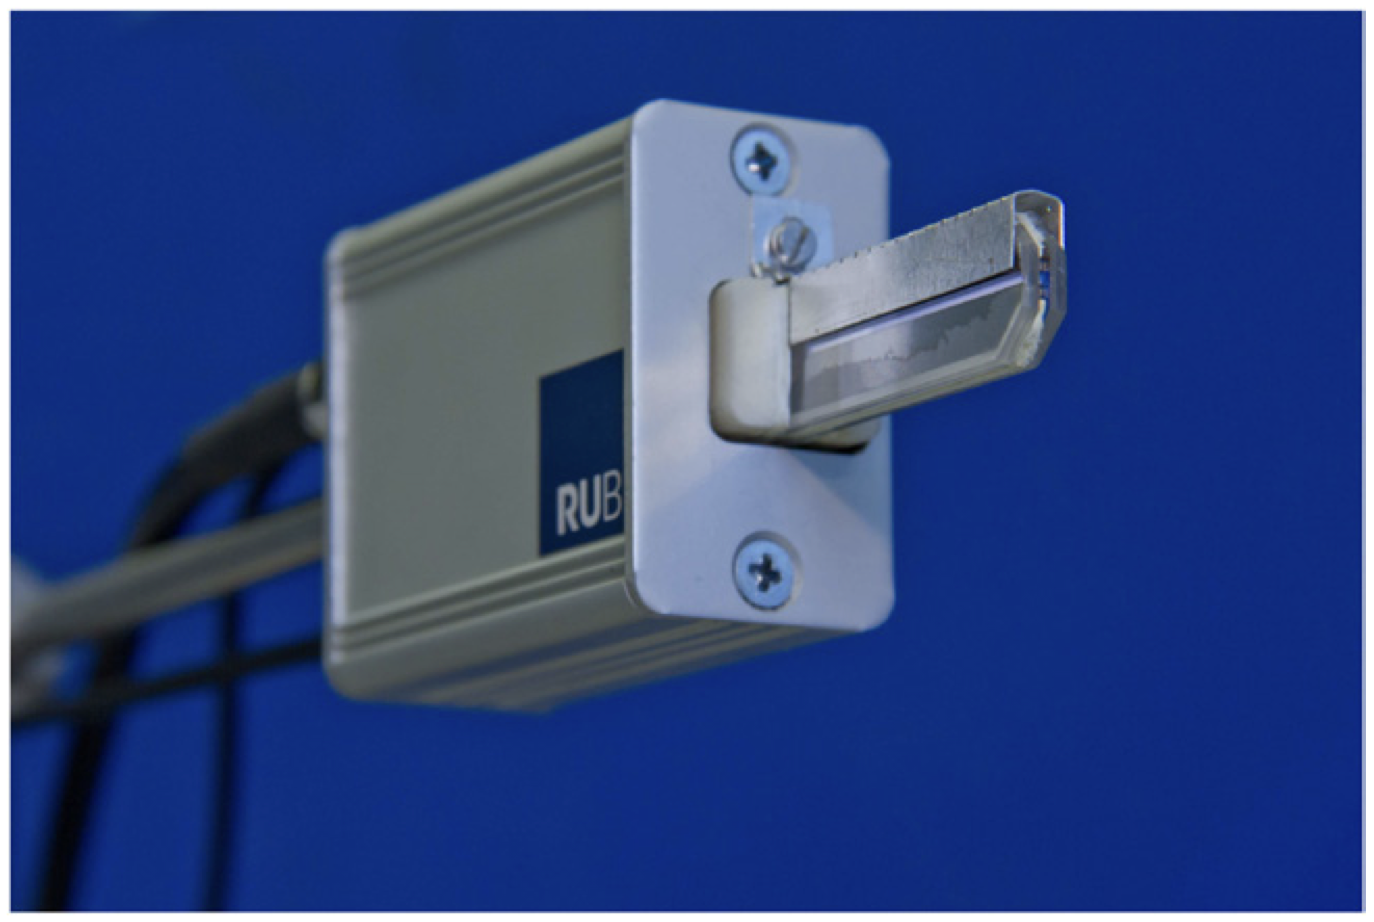
\includegraphics[width=0.75\linewidth]{chapter_3/figures/COST_jet.png}
	\caption{Photograph of COST jet \cite{Golda2016}.}
	\label{fig:COST_jet}
\end{figure}

Another more recent development was developed by  Xu et al \cite{Xu2021}. The reactor used was a COST microplasma jet developed by Schulz-von der Gathen et al \cite{VonDerGathen2008}, a capacitively coupled reactor that operated at 13.56 MHz. A picture of the jet can be seen in figure \ref{fig:COST_jet}, and the experimental setup by Xu et al is shown in figure \ref{fig:han_epoxidation_setup}. Their design also utilised a CO$_2$-He mixture, but with a co-reactant called \textit{trans}-stilbene. The the end product of this reaction was an epoxide (which is a popular compound use for detergents, adhesives, and plastics) and the waste gas CO. This reaction can be seen below:

\begin{equation}
    \ce{CO$_2$ + C_6H_5CH=CHC_6H_5 -> CO + epoxide}
\end{equation} 

\begin{figure}[h!]
	\centering
	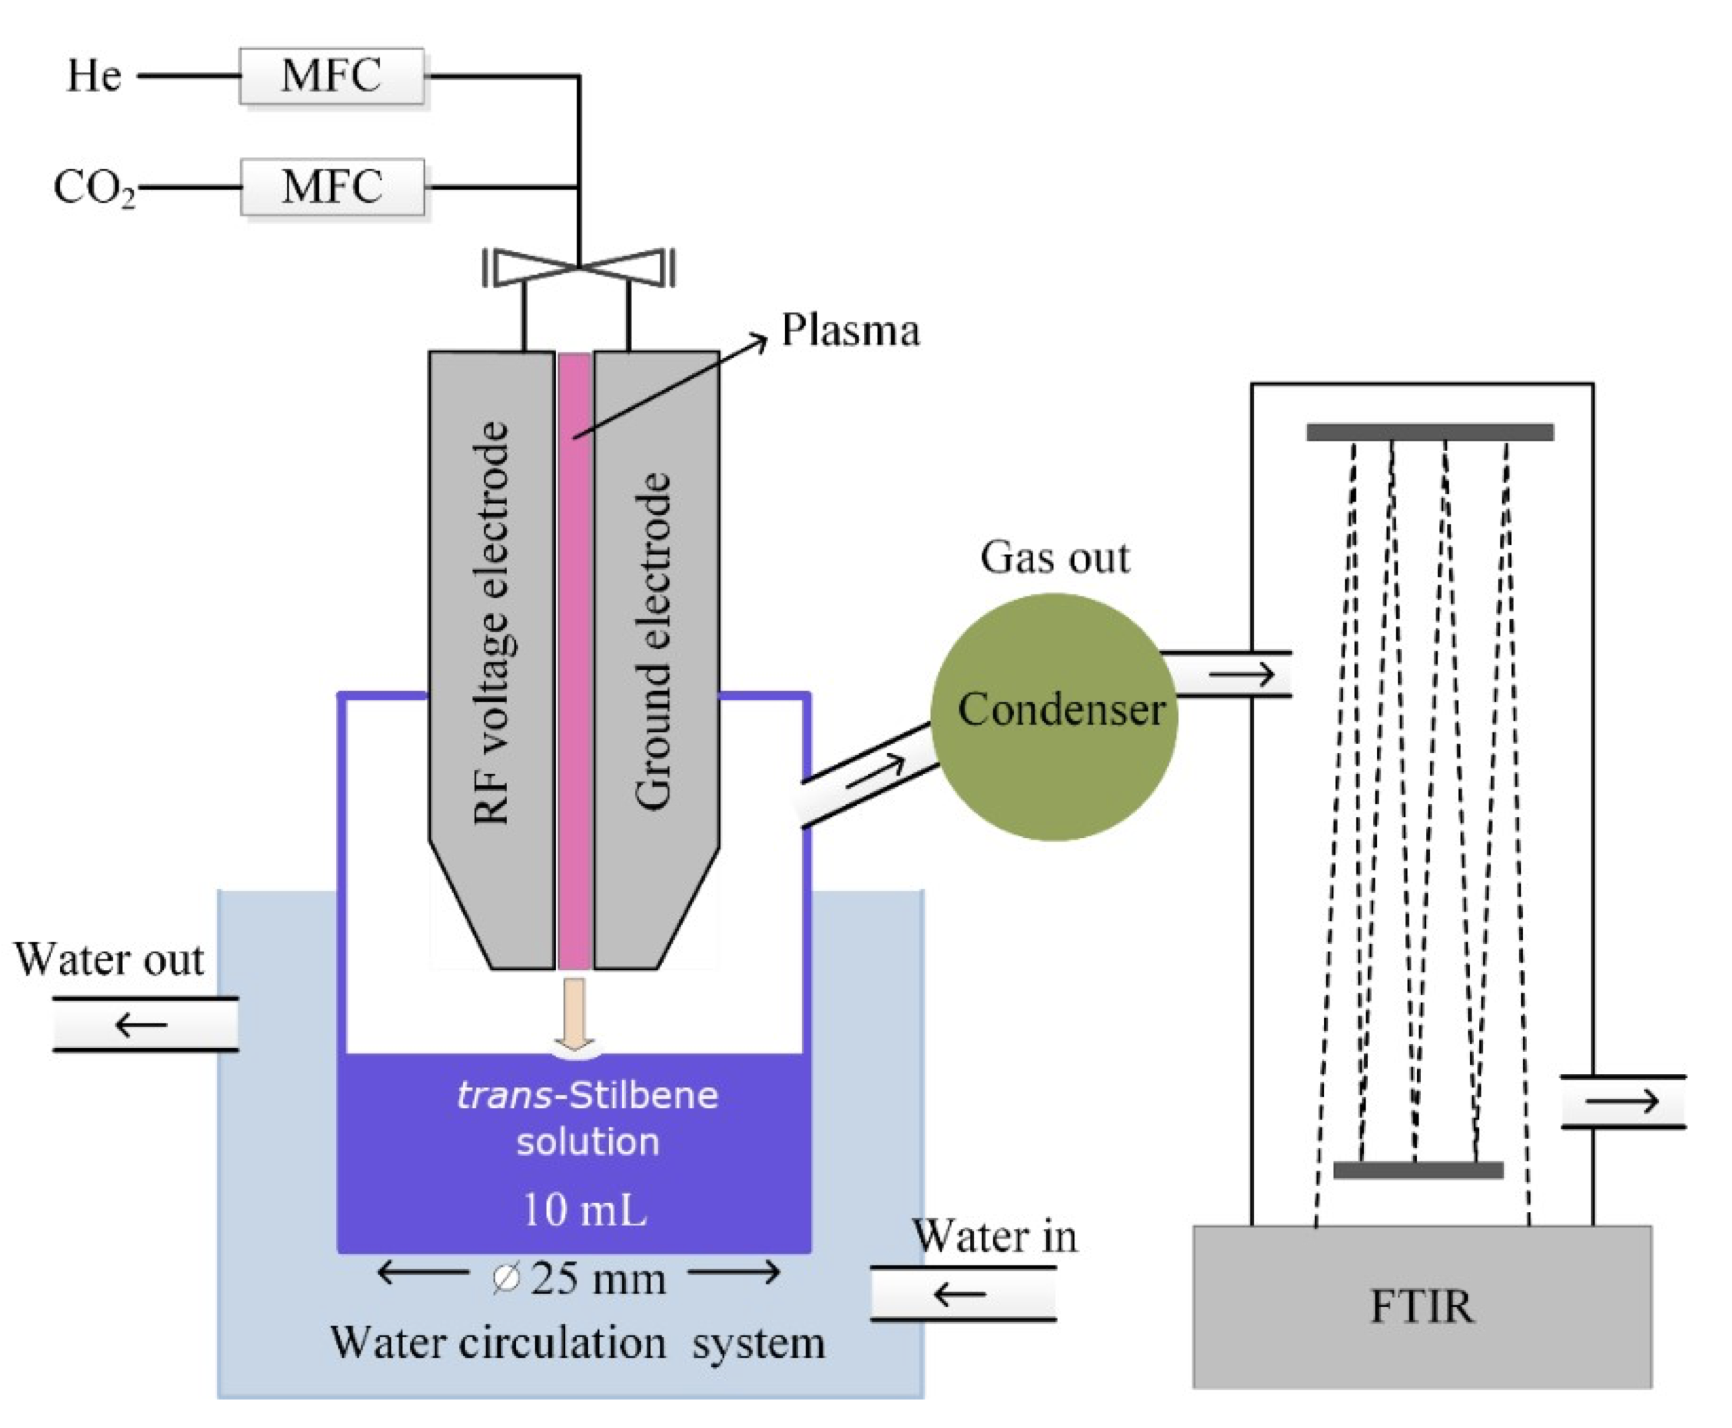
\includegraphics[width=0.75\linewidth]{chapter_3/figures/han_epoxidation_setup.png}
	\caption{Schematic of experimental setup by Xu et al \cite{Xu2021}.}
	\label{fig:han_epoxidation_setup}
\end{figure}


The plasma jet had to be placed 4 mm above the surface of the liquid, and the authors were able to reliably get yield on epoxides of around 75\%. The conversion efficiency was slightly lower at approximately 70\%. The authors did not provide an energy efficiency, and its value could not be determined as the details regarding the power of the reactor were not stated. 

This approach seems quite feasible especially considering it was operating at atmospheric pressure. The only downside of this process was that temperature seems to play a role in the efficiency of the reaction, with the best performance at around 250K. Nonetheless, the reaction is still perfectly viable at room temperature, with the yields dropping by only 5\%. As such, this will be the process that is emulated in this report.



 



%Nonetheless, other designs for RF/microwave discharges exist such as the one developed by Xu et al \cite{Xu2021}. Their design utilised a co-reactant called \textit{trans}-stilbene. Unlike the co-reactants previously mentioned, which were  gaseous, \textit{trans}-stilbene is a liquid. Because of this, the plasma had to directly contact the solution, which was achieved via a plasma jet reactor. The jet nozzle had to be place 4 mm above the surface of the liquid, and the final product of this reaction was CO and epoxides (a popular compound use for detergents, adhesives, and plastics). The authors were able to obtain a 75\% yield on epoxides and a splitting of approximately 70\% of the CO$_2$ in the plasma. As such, this will be the process that is emulated in this report.


